\documentclass[10pt,twocolumn,letterpaper]{article}

\usepackage{algorithmicx}
\usepackage{algorithm}
\usepackage{booktabs}
\usepackage{cvpr}
\usepackage{graphicx}
\usepackage{color, colortbl}
\usepackage{algpseudocode}
\usepackage{booktabs}
\usepackage{hyperref,url}
\usepackage{amsmath}
\usepackage[page]{appendix}

%Macros
\DeclareMathOperator*{\argmin}{arg\,min}
\DeclareMathOperator{\Corr}{Corr}

% List labels
\usepackage{scrextend}
\addtokomafont{labelinglabel}{\sffamily}

\renewcommand{\algorithmicrequire}{\textbf{Input:}}
\renewcommand{\algorithmicensure}{\textbf{Output:}}
\renewcommand{\thefootnote}{$\star$}

\cvprfinalcopy % *** Uncomment this line for the final submission

\usepackage{footmisc} % Daggers for author notes
\DefineFNsymbols{mySymbols}{{\ensuremath\dagger}{\ensuremath\ddagger}\S\P
   *{**}{\ensuremath{\dagger\dagger}}{\ensuremath{\ddagger\ddagger}}}
\setfnsymbol{mySymbols}

% Colors for highlighting tables
\definecolor{Gray}{gray}{0.9}

% Pages are numbered in submission mode, and unnumbered in camera-ready
%\ifcvprfinal\pagestyle{empty}\fi
\setcounter{page}{1}
\begin{document}

%%%%%%%%% TITLE
\title{Parallel \texttt{stable k-means}$^\star$}

\author{
    Emin Arakelian\thanks{\href{mailto:emin@berkeley.edu}{\nolinkurl{emin@berkeley.edu}}}
    \hspace{10mm}
    Fadi Kfoury\thanks{\href{mailto:fadi.kfoury@berkeley.edu}{\nolinkurl{fadi.kfoury@berkeley.edu}}}
    \hspace{10mm}
     Jason Poulos\thanks{\href{mailto:poulos@berkeley.edu}{\nolinkurl{poulos@berkeley.edu}}}
    \vspace{15mm}
}

\maketitle
%\thispagestyle{empty}

%%%%%%%%% ABSTRACT
\begin{abstract}
Abstract...
\end{abstract}

\footnotetext[1]{The code used for this project is available on Github: \url{https://github.com/plumSemPy/parallel_kmeans}.}

%\linenumbers

%% main text
\section{Introduction} \label{section:Intro}

Unsupervised learning is a branch of machine learning that infers patterns from data that has no labels. $k$-means is a popular unsupervised learning algorithm for finding clusters and cluster centers in data. The goal is to choose $k$ cluster centers to minimize the total squared distance between each data point and its closest center. In other words, its objective is to find

\[
\argmin_s \sum_{i=1}^{k}\sum_{x \in S_i}\parallel x - \mu_i \parallel^2.
\] Given $k$ initial centers chosen uniformly at random from the data points, $k$-means alternates between two steps until convergence: (\textit{assignment step}) each point is assigned to the nearest cluster center and; (\textit{update step}) each center is recomputed as the center of mass of all points assigned to it.

\
There are are several methods to determine the optimal number of clusters in unlabeled data. One way is to use different clustering metics such as the silhouette coefficient \cite{aranganayagi2007}. Another approach --- which is the subject of this project --- is stability \cite{ben2001}\cite{smith1980}. As we will later discuss, assessing stability requires multiple runs of $k$-means, which will make it computationally very expensive. Algorithms that speed up the selection of $k$ initial centers have been proposed, such as {\texttt{k-means++}}, which chooses only the first cluster center uniformly at random, and selects subsequent centers from the data points, weighed by a probability proportional to its contribution to the overall error \cite{arthur2007}. Bahmani et al. \cite{bahmani2012} propose a method of parallelizing the initialization that reduces the number of passes by sampling $O(k)$ points and for $O (\log n)$ rounds, instead of sampling a single point in each pass.\footnote{$k$-means is NP-hard, and can be solved in time  $O (n^{dk +1} \log n)$, where $n$ is the number of points in $d$ dimensions.}

Given that Python is one of the most popular coding languages for doing data science, we explore the options of parallelization of \texttt{stable k-means} in Python.\footnote{In this report by Python, Python 2 is meant and not Python 3.} We will take a look at our options in using parallelization in Python and analyze them briefly. As we will discover Python is not the ideal platform for parallel programming, so why bother? The reason is that Python is a very high level language with many good data types, databases, text parsing and many other capabilities that allow for complicated algorithms. One of the simplest functions we have in our \texttt{stable k-means} algorithm is generating an array of random numbers. In the snippet in Section \ref{py-compare} we see a comparison of this same task in C++ and Python. Thus it is a waste not to use Python's Parallel capabilities for speed ups, solely for the reason that they are not ideal. While we will mainly focus on Python in this project, it is entirely possible to use \texttt{Ctypes} in Python and get even higher performances using C extensions.

We describe the serial version of \texttt{stable k-means} in Section \ref{section:stable} and its parallel implementation using Python in Section \ref{parallel} . We then describe the implementation on simulated data in Section \ref{implementation}. We discuss challenges and future directions in Section \ref{challenges} and draw conclusions in Section \ref{conclusion}.

\section{Serial \texttt{stable k-means}} \label{section:stable}

%Ben-Hur et al. \cite{ben2001} propose an algorithm that uses stability of clustering with respect to perturbations such as sub-sampling to generate meaningful partitions of the data. The algorithm receives as input a dataset or similarity matrix and a parameter $k_{max}$ that sets the maximum number of clusters the algorithm produces. The algorithm measures stability for each value of $k \in 1 \ldots k_{max}$ using the distribution of pairwise similarities between clusterings from sub-sampled data, where high pairwise similarities indicate stable clustering. The algorithm compares the distribution of pairwise similarities for different values of $k$, and the optimal $k$ is chosen using the maximum value of the average similarity. 

Ben-Hur et al. \cite{ben2001} propose an algorithm for any clustering mechanism that will assess the stability of the points and thus let us infer the optimal number of clusters. The algorithm begins with subsampling the data twice with a ration more than half. It is believed that the general structure of the dataset is captured when subsampling with a ration bigger than a half. Then, for a given number of clusters, the two subsamples are clustered. The points in the intersection of the two subsamples are analyzed to see how many of them are clustered together in the same cluster in both subsamples. Then, depending on the number of the points clustered together in the intersection of both of the subsamples, a similarity score is calculated. We will use the correlation score for our application.

Let labeling $\mathcal{L}$ be a partition of $X$ into $k$ subsets $S_1, S_2, ... , S_k$. In that case the correlation score between the clustering of intersection of two subsamples is given by: 

\[
\Corr(\mathcal{L}_1, \mathcal{L}_2) = \frac{\langle \mathcal{L}_1, \mathcal{L}_2 \rangle}{\sqrt{\langle \mathcal{L}_1,\mathcal{L}_1\rangle \langle \mathcal{L}_2,\mathcal{L}_2\rangle}}
\]

The algorithm for \texttt{stable k-means} is displayed in Algorithm \ref{alg:stability}.

\begin{algorithm}[H] 
\textbf{Input}: $X$ \{a dataset\}, $k_{max}$ \{maximum number of
clusters\}, num\_subsamples \{number of subsamples\} 

\textbf{Output}: $S(i,k)$ \{list of similarities for each $k$ and
each pair of sub-samples\}

\textbf{Require}: A clustering algorithm: cluster$(X,k)$ ; a similarity
measure between labels: $s(\mathcal{L}_1,\mathcal{L}_2)$

1: $f = 0.7$ 

2: for $k=2$ to $k_{max}$ \textbf{do} 

3: for $i=1$ to $num_subsamples$ \textbf{do} 

4: $sub_1 = $subsamp$(X, f)$ \{a sub-sample with a fraction of $f$
the data\} 

5: $sub_2 = $subsamp$(X, f)$ 

6: $\mathcal{L}_1=$cluster$(sub_1, k)$ 

7: $\mathcal{L}_2=$cluster$(sub_2, k)$ 

8: Intersect $= sub_1 \cap sub_2$

9: $S(i, k) = s(\mathcal{L}_1(Intersect), \mathcal{L}_2(Intersect))$
\{Compute the similarity on the points common to both subsamples\} 

10: \textbf{end for }

11: \textbf{end for}

\caption{\label{alg:stability}}
\end{algorithm}

Given this algorithm, for each $k$, a distribution of scores will be attained. The distribution with the highest score and least variance is the best; distributions that are unimodal are also highly preferred. These criteria means that the consistently intersection points were clustered together and thus that certain formation of clusters was stable. 

\section{Parallelization} \label{parallel}

In this project we will be focusing on using Python's native multiprocessing module which accommodates multithreading and multiprocessing. In the following sections we will take a closer look on how each of the function.

\subsection{Threading and the GIL}

Python utilizes a multithreading module letting the user use multiple
threads. Python threads are real system threads, i.e. Posix threads
or Windows threads and are fully operated by the host operating system.
The caveat however is that for CPU-bound functions, the threaded version
will perform worse than the serial version. The reason behind that
is that parallel execution is forbidden in Python and there is a GIL,
Global Interpreter Lock, that ensures only one thread is ran at a
time in the interpreter which simplifies many of the low level tasks
like memory management and call out to C extensions. With the existence
of GIL we get a cooperative multitasking as shown in Figure \ref{fig:Cooperative-multitasking-with}.
When a thread is running it is holding the GIL and the GIL is released
upon I/O commands such as read, write, send, receive etc. Thus the
merit of multithreading will be apparent when the functions are I/O
bound. 

\begin{figure}[htbp] 
\begin{center}
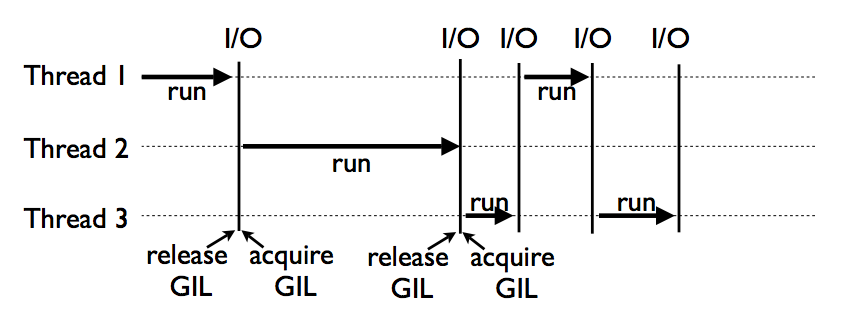
\includegraphics[scale=0.3]{figure/threads_IO.png}
\end{center}
\caption{Cooperative multitasking with GIL}
\label{fig:Cooperative-multitasking-with}
\end{figure}


CPU-bound threads that never perform I/O are handled differently where
there are special check for every 100 ``ticks'', see Figure \ref{fig:No-I/O-function}.
These ticks should not be confused with the clock ticks. These ticks
are roughly equivalent to one interpreter instruction. The check is
as follows, the current thread will reset the tick counter, reset
the signal handler if it is the main thread, release the GIL and reacquire
it.

\begin{figure}[htbp] 
\begin{center}
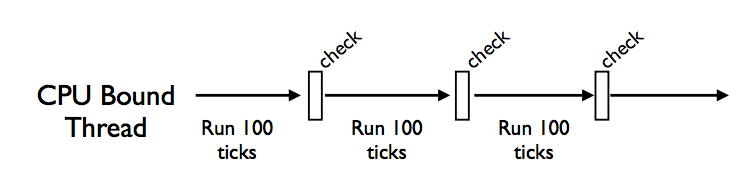
\includegraphics[scale=0.3]{figure/threads_check.png}
\end{center}
\caption{No I/O function checks}
\label{fig:No-I/O-function}
\end{figure}


In thread switching on a single core two cases can happen. Assume
we have two threads, with the first thread running. If at some point
the first thread has an I/O instruction, it will release the GIL and
the second thread will acquire it. However, if the first thread has
no I/O instructions, then the GIL release will happen on the check.
In which case the lock is free and two threads are ready to run. Here
the priority will be handled by the OS, and the next thread may or
may not be thread 2, however experimental result has shown that this
thread switching happens rarely, and there would be thousands of checks
before thread two will run. A more interesting problem arises when
multiple cores have runnable threads. Here the threads get scheduled
simultaneously on multiple cores and thus they will battle over the
GIL. This happens because when thread one releases the GIL and signals
universally, thread two takes some time to wake up to acquire the
lock, by which time thread one has acquired the lock and thread two,
failing at it's endeavors decides to sleep again. An illustration
is provided in Figure \ref{fig:GIL-wars-on}.

\begin{figure}[htbp] 
\begin{center}
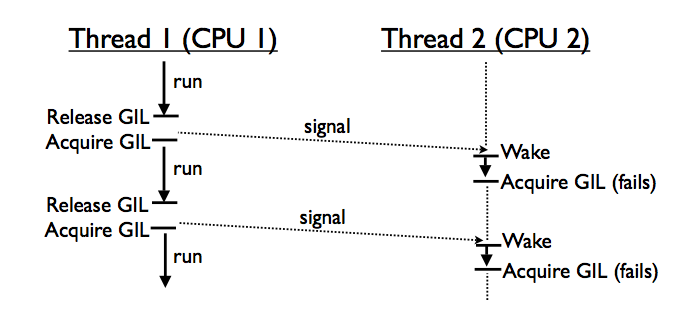
\includegraphics[scale=0.3]{figure/threads_multicore.png}
\end{center}
\caption{GIL wars on multicored threads}
\label{fig:GIL-wars-on}
\end{figure}


To remedy this problem, in Python 3 is a new GIL implementation that
allows thread two to signal a timeout in which case thread one will
drop the lock after its current instruction and thread two can take
over. This seems to address the problem a little, but still there
are starvation scenarios where the most deserving threads do not get
to run first due to scheduling. A suggested work around for this is
to separate CPU-bound, low priority threads and I/O, high priority
threads. 

In conclusion threading in Python has many caveats and edge cases
and must be dealt with cautiously. However it does provide improvements
that will be wasteful not to utilize.


\subsection{Multiprocessing}

A good alternative to multithreading is multiprocessing which came
about around Python 2.6. The syntax is exactly the same as multithreading
but here python uses processes instead of threads and thus eliminating
shared anything. Here we will have multiple instances of the interpreter
running each having their own GIL and the way they communicate is
message passing. The messages are being passed using ``pickle''-ing.
The pickle module in Python can serialize and deserialize python objects
into byte-streams. Since we are using message passing here, we can
deploy our code on multiple machines as well. 

\subsection{Other Python Parallel Libraries}
\begin{itemize}
\item \textbf{PyCUDA : }A Python wrapper for the CUDA API. \url{https://documen.tician.de/pycuda/}
\item \textbf{PyMPI : }An underdevelopment message passing interface for
Python being developed by Lawrence Livermore National Laboratory.
\url{http://pympi.sourceforge.net/}
\item \textbf{Asyncio : }Asynchronous I/O, event loop, coroutines and tasks.
\url{https://docs.python.org/3/library/asyncio.html}
\item \textbf{Twisted : }An event driven networking engine for Python. \url{https://twistedmatrix.com/trac/}
\end{itemize}
The latter two are trying to convert all the I/O handling into event,
and lean towards event driven programming and move away from threads
and processes.

\section{Experiments} \label{implementation}

We will run our algorithm and compare its results on a toy dataset
of 500 samples and 2 features. The dataset is plotted in Figure \ref{fig:Dataset-that-will}. The dataset is obviously split into 5 clusters at most. Running the
algorithm on this dataset will yield the following similarity scoring
distribution (Figure \ref{fig:Histograms-of-Similarity}).

\begin{figure}[htbp] 
\begin{center}
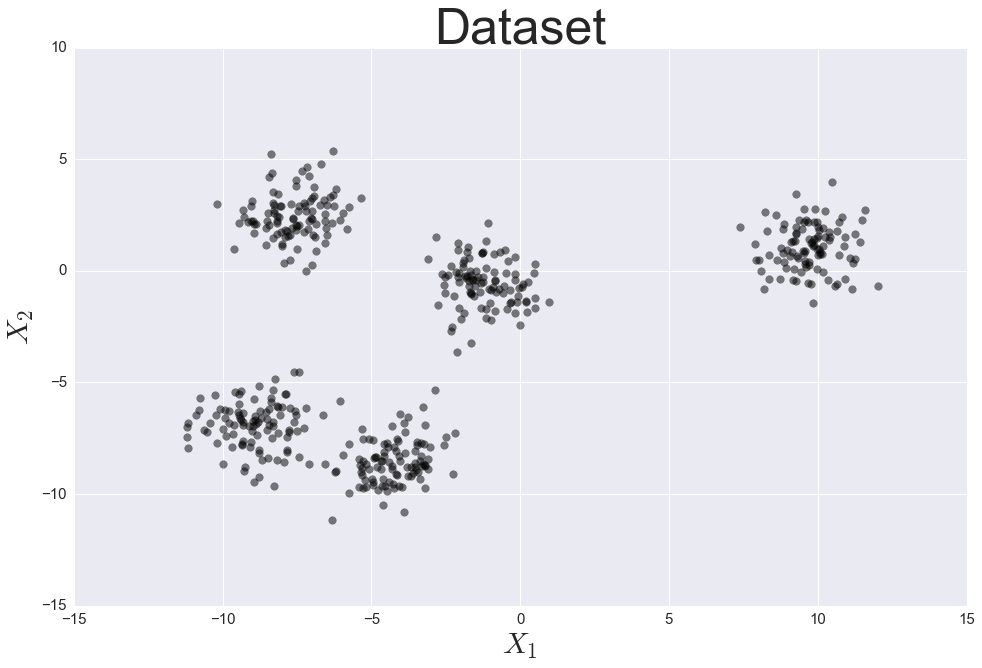
\includegraphics[scale=0.25]{figure/dataset.png}
\end{center}
\caption{\label{fig:Dataset-that-will}Dataset that will be used to assess
\texttt{stable k-means}}
\end{figure}


\begin{figure*}[htbp] 
\begin{center}
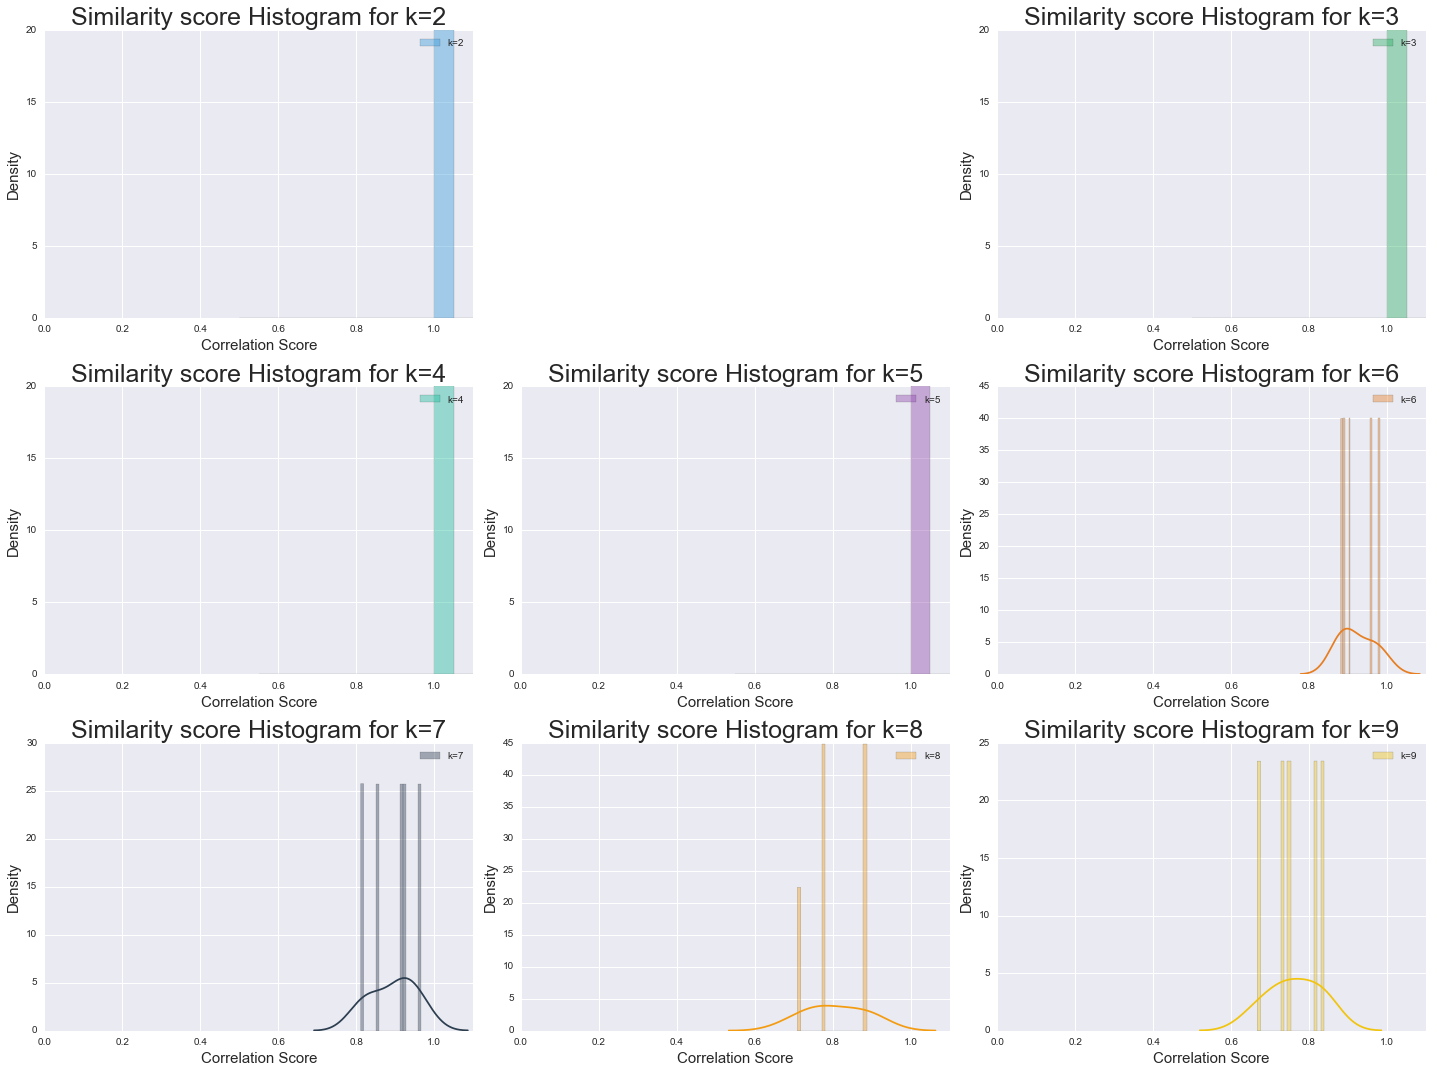
\includegraphics[scale=0.35]{figure/histogram.png}
\end{center}
\caption{\label{fig:Histograms-of-Similarity}Histograms of Similarity scores
for different ks.}
\end{figure*}


As seen the best results are given for 2 to 5 clusters.\footnote{The plots for 2 to 5 clustering formation is given in Section \ref{cluster-formation}.} It will be evident why we are getting such high scores on those cluster
formation, in other words why are those formations stable. 

We will now assess the runtime of our serial and parallel implementations.
In the parallel implementation we have parallelized the inner loop.
In that each process runs a subsampling, clustering and a similarity
scoring. They all then write their outputs to one shared array. Thus
each processes or thread will run number\_of\_samples/(number\_of\_processes
or number\_of\_threads) times. Figure \ref{fig:Serial-Run-Time} shows
the baseline serial run time. The time complexity of $k$-means is $O(n^{dk+1}\log n$.
Since we are doing a loop over $k=2$ to$ k=K$ then our complexity will
go to $O(n^{dk_1}+n^{dk_2}+ ... +n^{dK})n \log n$. Note that the fact
that we run in num\_subsamples does not affect the time complexity. 

\begin{figure}[htbp] 
\begin{center}
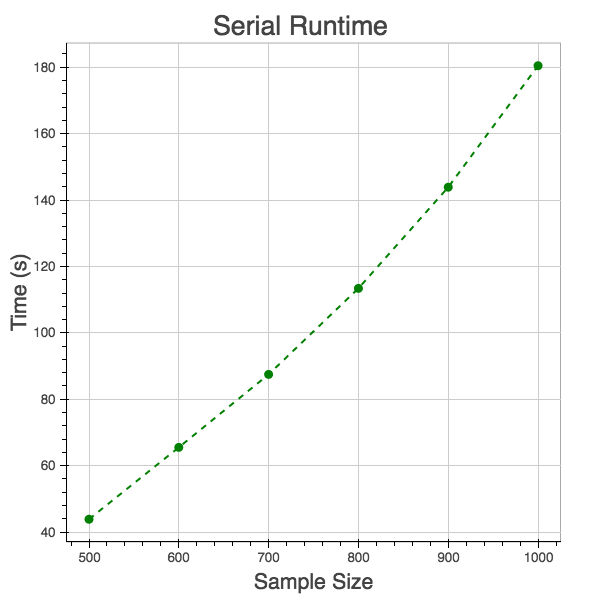
\includegraphics[scale=0.35]{figure/serial.png}
\end{center}
\caption{\label{fig:Serial-Run-Time}Serial Run Time}
\end{figure}


Figure \ref{fig:Strong-and-Weak} shows the strong and weak scaling
of the multithread and multiprocess algorithms. As evident the optimal
number of threads and processes are attained at 3 threads and 3 processes.
After that the code starts getting slow most likely because the machine
that this code was run on had 4 cores. As expected, since the code
is I/O bound, threading improved the run time, but not as much as
multiprocessing, where concurrency of the threading is replaced by
parallelization. Sadly since we do net yet have access to more cores
we aren't able to tune the size up to attain a good weak scaling.
It looks as though the OS is scheduling one process or thread per
core and hence the speedups and speed downs.

\begin{figure}[htbp] 
\begin{center}
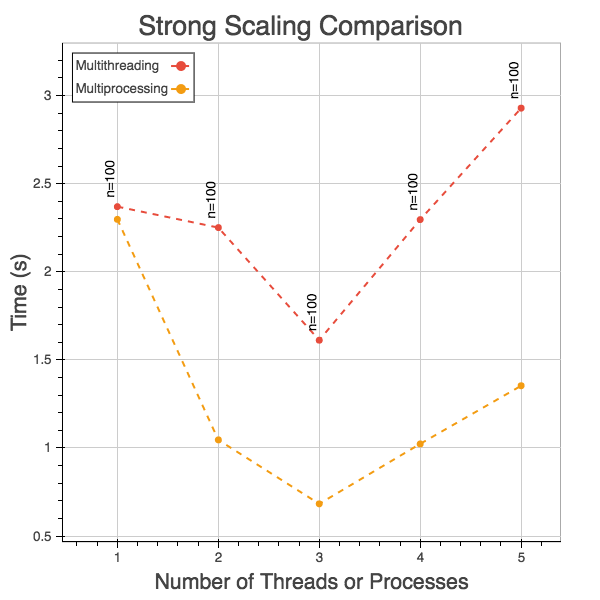
\includegraphics[scale=0.35]{figure/mt_mp_ss_comp.png} \\
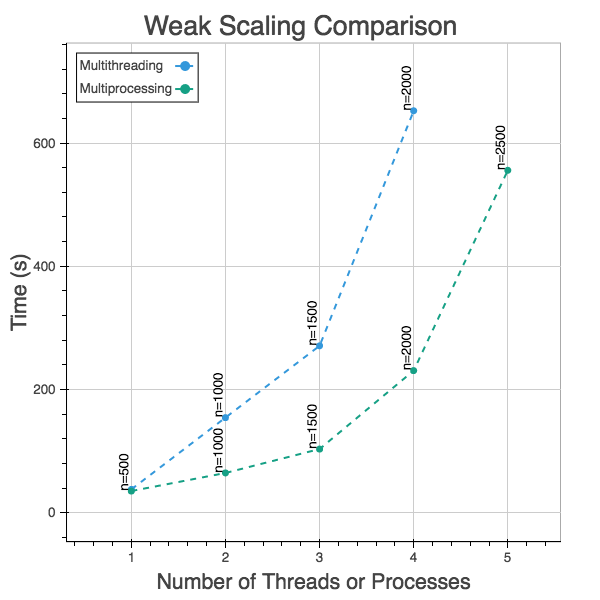
\includegraphics[scale=0.35]{figure/mt_mp_ws_comp.png}
\end{center}
\caption{\label{fig:Strong-and-Weak}Strong and Weak Scaling Comparison for
Multithreading and Multiprocessing}
\end{figure}


Figure \ref{fig:Speed-up-Comparison} below shows a comparison of
the run time on the serial, concurrent (multithread) and parallel
(multiprocess) code. The sample size varies between 100 to 500 samples
and 3 threads and processes are taken to do the comparison as they
were the optimal on the previous part. From the serial implementation
and 500 samples we have a 1.3 times speed up for the multithread algorithm
and a 3.3 times speed up for the multiprocess algorithm.

\begin{figure}[htbp] 
\begin{center}
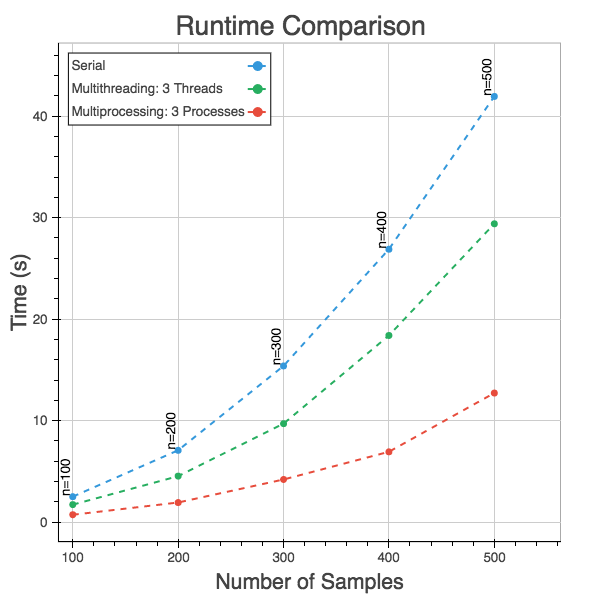
\includegraphics[scale=0.35]{figure/runtime_comparison.png}
\end{center}
\caption{\label{fig:Speed-up-Comparison}Speed up Comparison}
\end{figure}


\section{Challenges and Future Directions} \label{challenges}

One of the first challenges faced was the lack of proper documentation
on many of the Python's parallel libraries. We were initially decided
to include GPUs by using CUDA as a comparison here. But due to the
huge difficulty of installing CUDA on the only Nvidia machine we had,
and given that we want to make this package available for public use,
we revised and decided to hold off on CUDA for now until a much more
user friendly installation pipeline is provisioned. The pyMPI package
seems promising but it is still under development.

As mentioned earlier the multiprocessing module uses pickles to send
messages. Our implementation parallelizes a method in a class in Python
and unfortunately pickle cannot pickle a class instance method. For
that we had to use a fork of the multiprocessing called \texttt{pathos.multiprocessing}
which uses ``dill'' instead of ``pickle''. 

There might be some speedups, if we collect the results from each
process separately and then put them in the global array, instead
of asking them to write their result at the end of each $k^{th}$ iteration.
A profiling of the method shows that significant time is spent in
waiting and acquiring the lock to write to the array.

In terms of scalability of the memory, one improvement might be possible
if instead of giving each process an entire copy of the data, we put
the jobs in a queue and ask each process to take its job from there,
or alternatively we can send them their jobs. But that might result
in increased waiting times on the lock again to get the job from the
queue.


\section{Conclusion} \label{conclusion}

Python is a hugely popular platform for performing very high level
complex algorithms. The merit being the fact that the programmer needs
to spend less time worrying about optimization and tweaking the little
knobs and spend more time on creating something more complex. Python
is infamous for its GIL and threading problems. The creators of Python
wanted to simply their low level managements by avoiding shared anything.
That should not however prevent us from trying to get the best out
of the language, especially with the advent of the new multiprocessing
library. PyCUDA and pyMPI show a lot of promise, however CUDA really
needs to revamp its use pipeline. We attempted parallelizing a very
useful algorithm that returns the optimal number of clusters in a
given dataset. The results show that we can attain very decent speed-ups using multiprocessing on an average machine.

{\small
\bibliographystyle{ieee}
\bibliography{refs}
}

\clearpage
\begin{appendices}

\section{Python vs. C++ comparison} \label{py-compare} 

\begin{verbatim}
C++
#include <algorithm>
#include <cstdlib>
#include <iostream>scale=0.35

int main() {
    int a[8] = {0, 1, 2, 3, 4, 5, 6, 7};     
	std::srand(unsigned(std::time(0)));
    std::random_shuffle(a, a + 8);
    for (int i=0; i<8; i++)         
	std::cout << a[i] << " "; std::cout << std::endl; }

Python 
import random
import numpy as np

random_array = np.array(random.sample(range(8),8))
\end{verbatim}

\section{Cluster formation} \label{cluster-formation}

Figure \ref{fig:2-Clusters-Formation}, \ref{fig:3-Clusters-Formation}
, \ref{fig:4-Cluster-Formation} , \ref{fig:5-Cluster-Formation}
, \ref{fig:6-Cluster-Formation} show why 2 to 5 clusters are stable
for our toy dataset and 6 clusters is not. We can see in the figures
that there is a clear grouping between 2, 3, 4 and 5 clusters. Thus
certain points always cluster together. However for 6 clusters, one
of the obvious clusters needs to split into 2, and that is an arbitrary
choice and hence the non-unimodal histograms.

\begin{figure}[htbp] 
\begin{center}
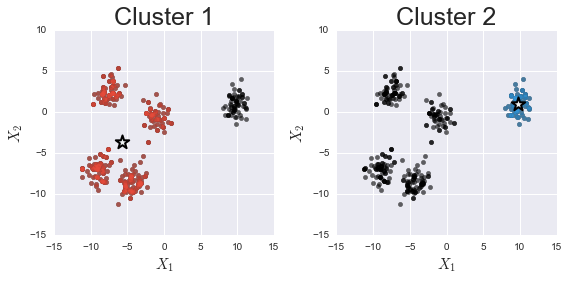
\includegraphics[scale=0.45]{figure/2_formation.png}
\end{center}

\caption{\label{fig:2-Clusters-Formation}2 Clusters Formation}


\end{figure}


\begin{figure*}[htbp] 
\begin{center}
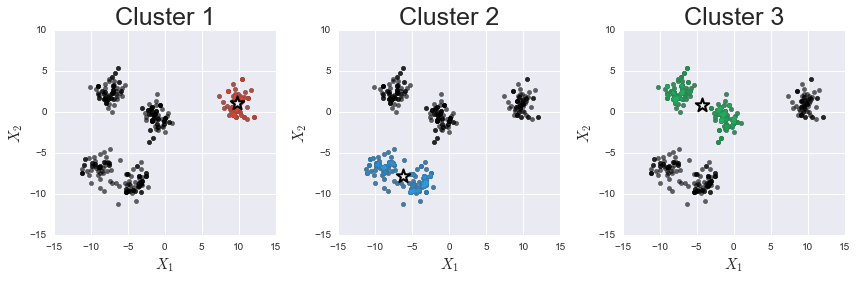
\includegraphics[scale=0.45]{figure/3_formation.png}
\end{center}

\caption{\label{fig:3-Clusters-Formation}3 Clusters Formation}
\end{figure*}


\begin{figure*}[htbp] 
\begin{center}
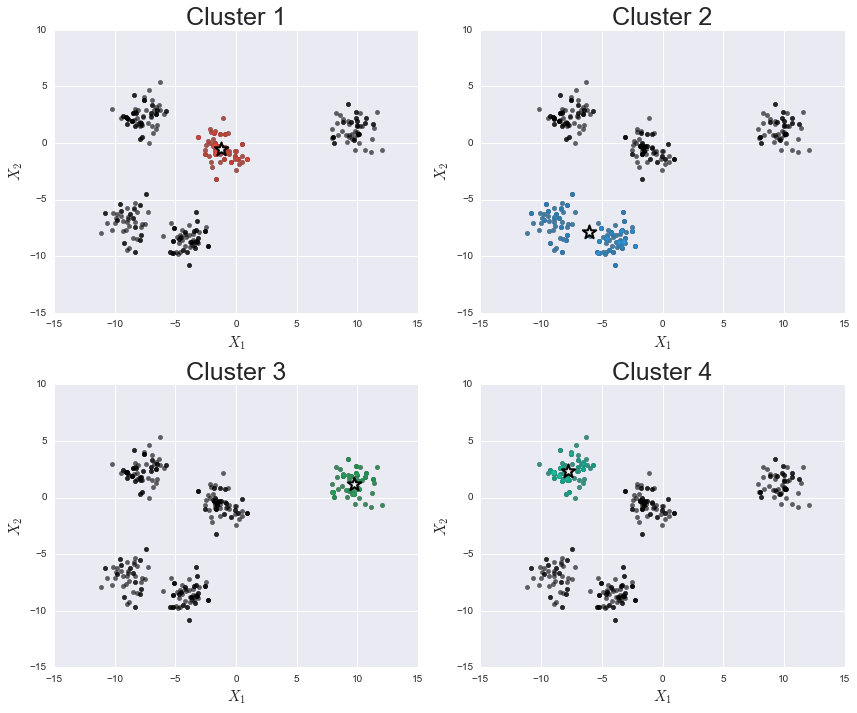
\includegraphics[scale=0.45]{figure/4_formation.png}
\end{center}

\caption{\label{fig:4-Cluster-Formation}4 Cluster Formation}


\end{figure*}


\begin{figure*}[htbp] 
\begin{center}
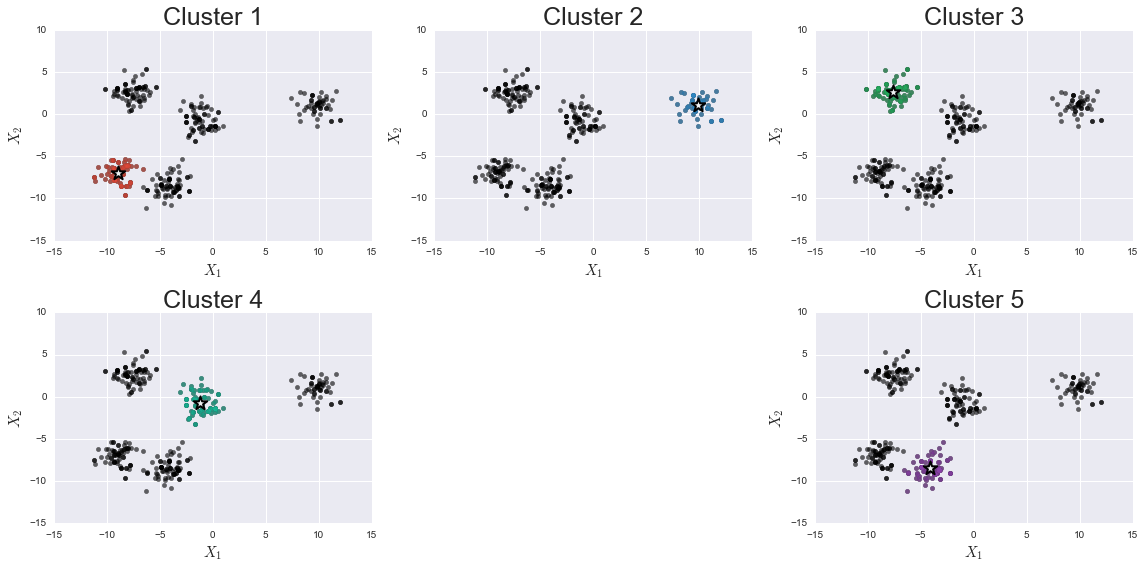
\includegraphics[scale=0.45]{figure/5_fomration.png}
\end{center}

\caption{\label{fig:5-Cluster-Formation}5 Cluster Formation}


\end{figure*}


\begin{figure*}[htbp] 
\begin{center}
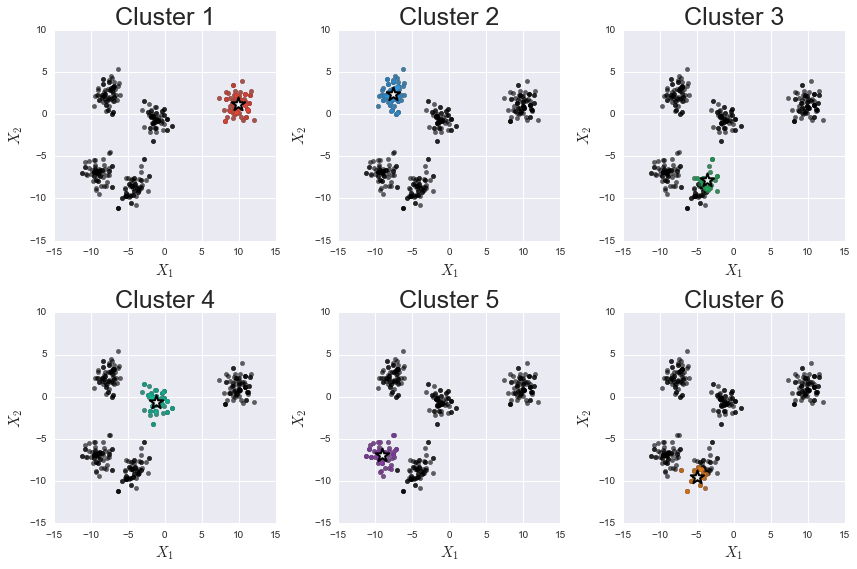
\includegraphics[scale=0.45]{figure/6_formation.png}
\end{center}

\caption{\label{fig:6-Cluster-Formation}6 Cluster Formation}


\end{figure*}

\end{appendices}

\end{document}
